\documentclass{standalone}
\usepackage{tikz}
\usetikzlibrary{patterns}
\usetikzlibrary{positioning}
\usetikzlibrary{patterns, positioning}
\usetikzlibrary{shapes.misc}
\usepackage[outline]{contour}
\contourlength{1.5pt} 
\usepackage[sfdefault]{ClearSans}

\begin{document}
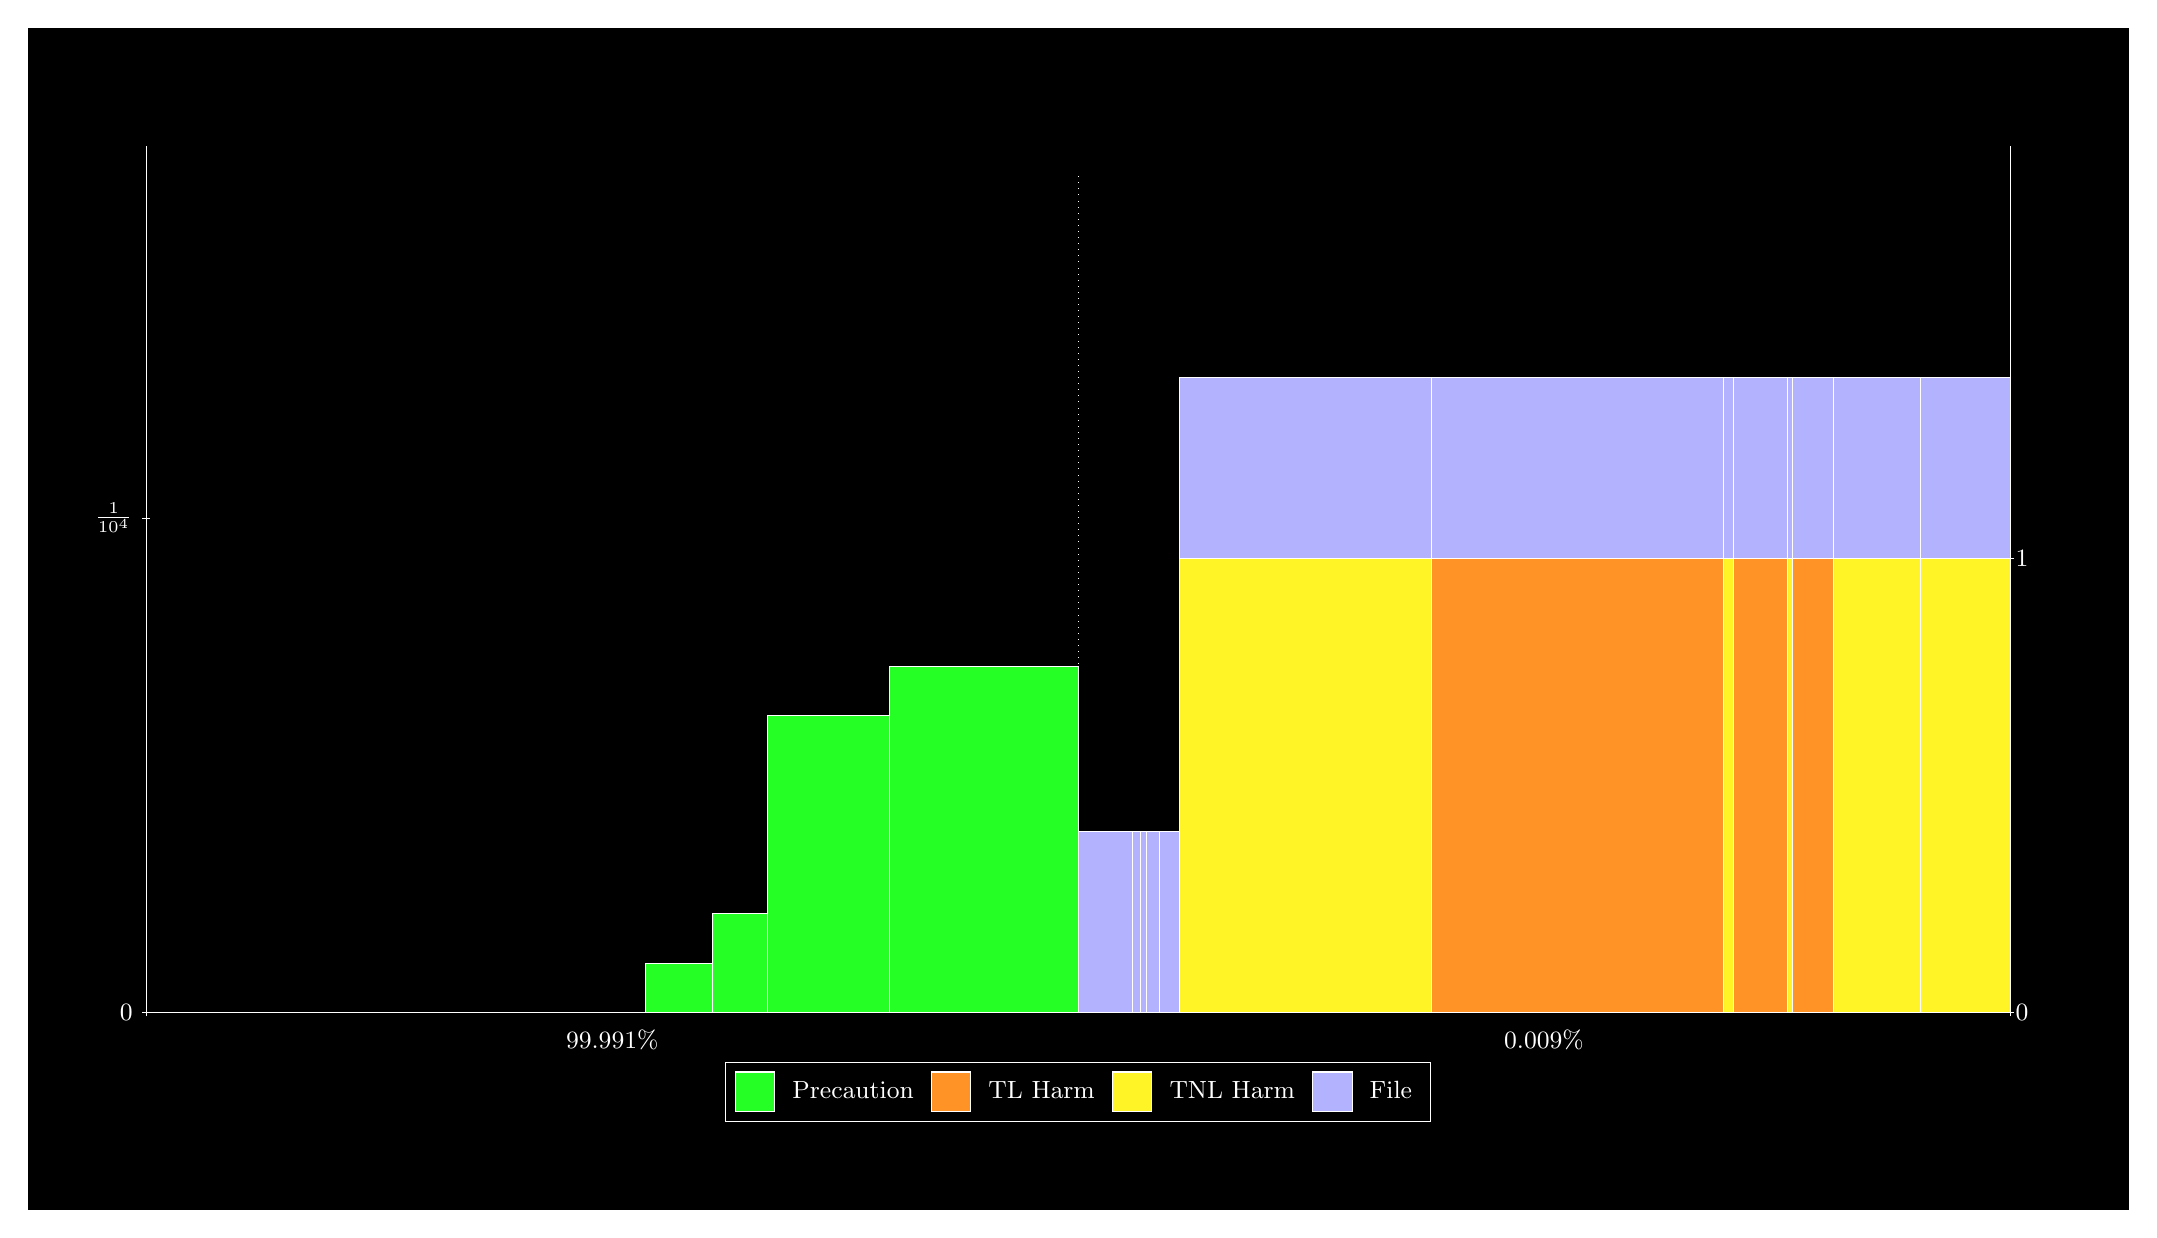
\begin{tikzpicture}
\draw[fill=black] (0,0) rectangle (26.667,15);
\draw[fill=green!85,draw=white,very thin] (7.8418,2.5) rectangle (8.6891,3.1282);
\draw[fill=green!85,draw=white,very thin] (8.6891,2.5) rectangle (9.3888,3.7564);
\draw[fill=green!85,draw=white,very thin] (9.3888,2.5) rectangle (10.936,6.2692);
\draw[fill=green!85,draw=white,very thin] (10.936,2.5) rectangle (13.333,6.8974);
\draw[fill=blue!30,draw=white,very thin] (13.333,2.5) rectangle (14.024,4.8066);
\draw[fill=green!85,draw=white,very thin] (14.024,2.5) rectangle (14.117,2.5001);
\draw[fill=blue!30,draw=white,very thin] (14.024,2.5001) rectangle (14.117,4.8066);
\draw[fill=green!85,draw=white,very thin] (14.117,2.5) rectangle (14.193,2.5001);
\draw[fill=blue!30,draw=white,very thin] (14.117,2.5001) rectangle (14.193,4.8067);
\draw[fill=green!85,draw=white,very thin] (14.193,2.5) rectangle (14.361,2.5003);
\draw[fill=blue!30,draw=white,very thin] (14.193,2.5003) rectangle (14.361,4.8069);
\draw[fill=green!85,draw=white,very thin] (14.361,2.5) rectangle (14.622,2.5004);
\draw[fill=blue!30,draw=white,very thin] (14.361,2.5004) rectangle (14.622,4.807);
\draw[fill=yellow!85,draw=white,very thin] (14.622,2.5) rectangle (17.819,8.2664);
\draw[fill=blue!30,draw=white,very thin] (14.622,8.2664) rectangle (17.819,10.573);
\draw[fill=orange!85,draw=white,very thin] (17.819,2.5) rectangle (21.532,8.2664);
\draw[fill=blue!30,draw=white,very thin] (17.819,8.2664) rectangle (21.532,10.573);
\draw[fill=green!85,draw=white,very thin] (21.532,2.5) rectangle (21.658,2.5001);
\draw[fill=yellow!85,draw=white,very thin] (21.532,2.5001) rectangle (21.658,8.2665);
\draw[fill=blue!30,draw=white,very thin] (21.532,8.2665) rectangle (21.658,10.573);
\draw[fill=green!85,draw=white,very thin] (21.658,2.5) rectangle (22.345,2.5001);
\draw[fill=orange!85,draw=white,very thin] (21.658,2.5001) rectangle (22.345,8.2665);
\draw[fill=blue!30,draw=white,very thin] (21.658,8.2665) rectangle (22.345,10.573);
\draw[fill=green!85,draw=white,very thin] (22.345,2.5) rectangle (22.399,2.5001);
\draw[fill=yellow!85,draw=white,very thin] (22.345,2.5001) rectangle (22.399,8.2666);
\draw[fill=blue!30,draw=white,very thin] (22.345,8.2666) rectangle (22.399,10.573);
\draw[fill=green!85,draw=white,very thin] (22.399,2.5) rectangle (22.92,2.5001);
\draw[fill=orange!85,draw=white,very thin] (22.399,2.5001) rectangle (22.92,8.2666);
\draw[fill=blue!30,draw=white,very thin] (22.399,8.2666) rectangle (22.92,10.573);
\draw[fill=green!85,draw=white,very thin] (22.92,2.5) rectangle (24.033,2.5003);
\draw[fill=yellow!85,draw=white,very thin] (22.92,2.5003) rectangle (24.033,8.2668);
\draw[fill=blue!30,draw=white,very thin] (22.92,8.2668) rectangle (24.033,10.573);
\draw[fill=green!85,draw=white,very thin] (24.033,2.5) rectangle (25.167,2.5004);
\draw[fill=yellow!85,draw=white,very thin] (24.033,2.5004) rectangle (25.167,8.2668);
\draw[fill=blue!30,draw=white,very thin] (24.033,8.2668) rectangle (25.167,10.573);
\draw[white,very thin] (1.5,2.5) -- (1.5,13.5);
\draw[white,very thin] (1.45,2.5) -- (1.55,2.5);
\node[font=\small,text=white, anchor=east] at (1.45, 2.5) {0};
\draw[white,very thin] (1.45,8.782) -- (1.55,8.782);
\node[font=\small,text=white, anchor=east] at (1.45, 8.782) {$\frac{1}{10^{4}}$};

\draw[white,dotted,very thin] (13.333,2.83) -- (13.333,13.17);
\draw[white,very thin] (25.167,2.5) -- (25.167,13.5);
\draw[white,very thin] (25.117,2.5) -- (25.217,2.5);
\node[font=\small,text=white, anchor=west] at (25.117, 2.5) {0};
\draw[white,very thin] (25.117,8.2664) -- (25.217,8.2664);
\node[font=\small,text=white, anchor=west] at (25.117, 8.2664) {1};

\draw[white,very thin] (1.5,2.5) -- (25.167,2.5);
\draw[white,very thin] (1.5,2.45) -- (1.5,2.55);
\node[font=\small,text=white, anchor=north] at (1.5, 2.45) {};
\draw[white,very thin] (25.167,2.45) -- (25.167,2.55);
\node[font=\small,text=white, anchor=north] at (25.167, 2.45) {};

\node[font=\small,text=white,anchor=south] at (7.4167, 1.9) {99.991\%};
\node[font=\small,text=white,anchor=south] at (19.25, 1.9) {0.009\%};
\draw (13.3333,2.5) node (B) {};
\begin{scope}[align=center]
\matrix[scale=0.5,draw=white,below=0.5cm of B,nodes={draw},column sep=0.1cm]{
\node[rectangle,draw,minimum width=0.5cm,minimum height=0.5cm,fill=green!85]{}; & \node[draw=none,font=\small,text=white]{Precaution}; &
\node[rectangle,draw,minimum width=0.5cm,minimum height=0.5cm,fill=orange!85]{}; & \node[draw=none,font=\small,text=white]{TL Harm}; &
\node[rectangle,draw,minimum width=0.5cm,minimum height=0.5cm,fill=yellow!85]{}; & \node[draw=none,font=\small,text=white]{TNL Harm}; &
\node[rectangle,draw,minimum width=0.5cm,minimum height=0.5cm,fill=blue!30]{}; & \node[draw=none,font=\small,text=white]{File}; \\\\
};\end{scope}

\end{tikzpicture}
\end{document}